\begin{mdframed}
    \textbf{La extensión máxima para esta sección es de 4 páginas.}
\end{mdframed}

\begin{figure}[H]
    \centering
    \begin{minipage}[t]{0.5\textwidth}
        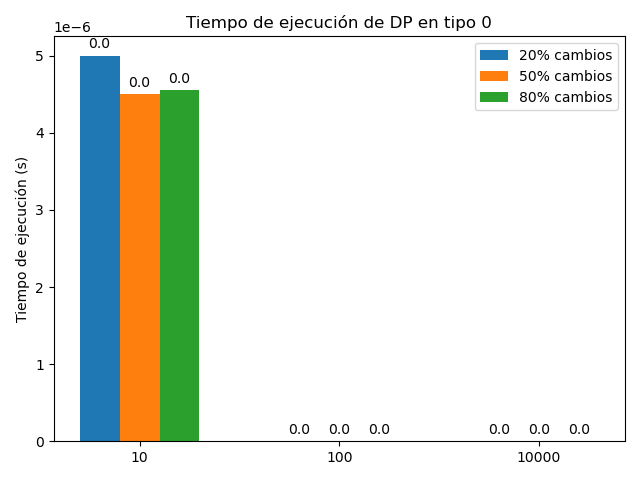
\includegraphics[width=\textwidth]{images/0_bruteforce.png}
    \end{minipage}%
    \begin{minipage}[t]{0.5\textwidth}
        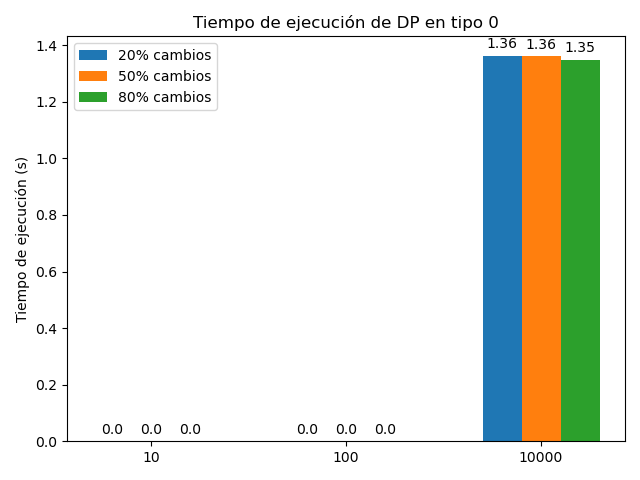
\includegraphics[width=\textwidth]{images/0_dp.png}    \end{minipage}%
    \caption{Tiempo de ejecución de los algoritmos en base a carácteres exclusivamente en mayúscula.}
    \label{fig:scatterplot_3}
\end{figure}

\begin{figure}[H]
    \centering
    \begin{minipage}[t]{0.5\textwidth}
        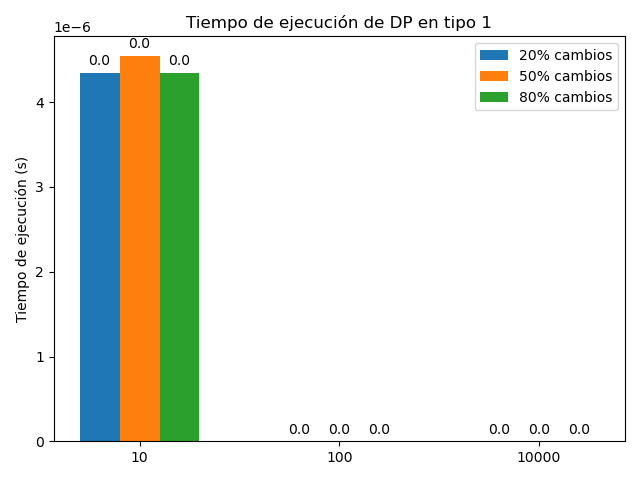
\includegraphics[width=\textwidth]{images/1_bruteforce.png}
    \end{minipage}%
    \begin{minipage}[t]{0.5\textwidth}
        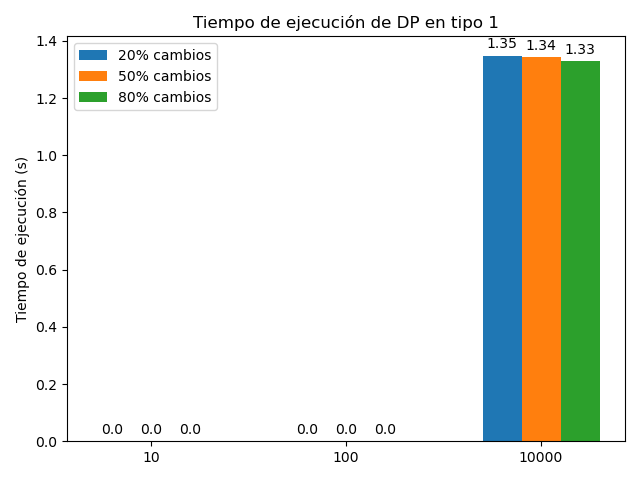
\includegraphics[width=\textwidth]{images/1_dp.png}    \end{minipage}%
    \caption{Tiempo de ejecución de los algoritmos en base a carácteres en mayúscula y en minúscula.}
    \label{fig:scatterplot_3}
\end{figure}

El algoritmo bruteforce sale con tiempo de ejecución 0 para N = 100 y N = 10000. Esto es porque luego de intentar correrlo con un par de strings de tamaño 100, no terminaba de calcular nunca; esto es debido a su complejidad de tiempo antes discutida en el análisis algorítmico (sección 2 del informe). Por tanto, solo se procesaron sus tiempos de ejecución para N = 10.

Notar que incluso para valores chicos de N como 10, el algoritmo de DP ya supera al algoritmo de fuerza bruta, pese a que el primero debe construir la tabla de DP antes de empezar a ejecutar. Esto es tanto un testamento a la rapidez del DP como también la ineficiencia del enfoque de fuerza bruta para este particular algoritmo; si bien no se nota en los gráficos ya que ambos son rondeados a 0.0, examinando las mediciones exactas en las carpetas de measurements, se llega a ver que el algoritmo de DP llega a ser entre 2 y 100 veces más rápido que el de fuerza bruta, particularmente cuando la diferencia entre strings es alta.

Para valores más grandes, como hemos dicho anteriormente, el algoritmo de fuerza bruta no termina de correr nunca. Para N = 100, el algoritmo de DP se ejecuta casi instantaneamente (al punto de quedar nuevamente aproximado a 0.0 en el gráfico), mientras que para N = 10000, se demora poco más de un segundo.

Cabe mencionar que se intentó ejecutar el algoritmo de DP para N = 100000 y N = 1000000, pero no se pudo debido a que la complejidad espacial del algoritmo provoca que se llene la memoria del computador el momento que se intentan procesar pares de string de estos tamaños, aspecto mencionado anteriormente en el análisis del algoritmo. En particular, sólo para N = 100000, la cantidad de memoria requerida para construir la tabla de DP es de (100000*100000*4bytes) = \textbf{37,2 gigabytes} de memoria. Para referencia, mi sistema es de sólo 16GB de RAM, y muchos computadores modernos llegan a tener como mucho 32GB de RAM; algunos sistemas entusiastas tienen 64GB, menos del doble de la cantidad de memoria requerida. Para N = 1000000, ni hablar.


\begin{mdframed}
    Recuerde que es imprescindible que se pueda replicar la generación de las gráficas, por lo que usted debe incluir cómo generó esos datos y  cómo podría generarlos la persona que revisa su entrega y ejecuta sus programas. Por ejemplo, si genera un scatterpolot con Tikz, usted debe explicar cómo obtener la tupla de valores que se usaron para generar la gráfica.
\end{mdframed}
